\documentclass{article}
\usepackage{graphicx}
\usepackage{float}
\usepackage[acronym]{glossaries}
\usepackage{fullpage}

\loadglsentries{acronyms}
\makeglossaries

\begin{document}

\begin{tabular}{rl}
  \textbf{Lab 7:} & DC Motor Configurations \\
  \textbf{Performed:} & March 11, 2013 \\
  \textbf{Partners:} & Rawley Dent \\ & Charles Pittman \\
  \textbf{Instructor:} & Dr. Weatherford
\end{tabular}

%\setlength\parindent{0pt}

\section*{Abstract}

%In this experiment, the operating characteristics of a separately excited DC
%motor were analyzed.  This report highlights two parts: the investigation of
%the relationship between motor torque and armature current, and the
%investigation of DC motor saturation effects.  To determine the relationship
%between the motor torque and armature current, the load torque at the
%dynanometer was increased while the voltage supply was held at 116.5-V.  The
%motor torque and resulting armature current was then recorded and analyzed.
%To determine the DC motor saturation effect, the field current was increased
%using the field control rheostat while the armature current was held at 1.5-A.
%The field current and resulting output torque was then recorded and analyzed.

\section*{Results}

\begin{figure}[H]
  \centering
    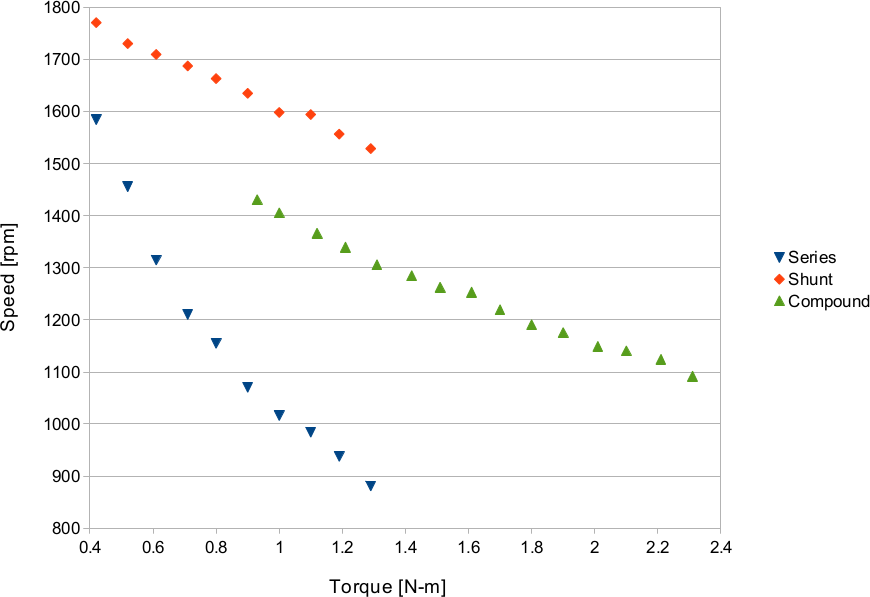
\includegraphics[width=0.6\textwidth]{img/graph}
    \caption{\textbf{Comparison of Speed vs. Torque Plots}}
    \label{fig:graph}
\end{figure}

\section*{Conclusions}

In Figure~\ref{fig:graph}, the linear relationship between DC motor speed $n_m$
and torque $\tau$ is exemplified.  The DC motor was initially operating at
approximately 1500-rpm.  As the load torque was increased, the DC motor
experienced a decrease in speed.  The armature current was also increasing
while the load torque was increasing, and thus the internal generated voltage
$E_A$ was decreased.

In Figure~\ref{fig:graph}, the DC motor saturation effects are shown.  This
plot is similar to a DC motor magnetization curve, where the field current is
plotted against the internal voltage.  Here, the field current was plotted
against the output torque.  Since the torque in any real machine depends on the
flux in the machine, and the internal voltage $E_A$ is directly proportional to
the flux produced, the y-axis in Figure~\ref{fig:graph} can be represented by
torque and not $E_A$ as in a DC machine magnetization curve.  This plot shows
that initially a large increase in field current correlates to a sharp increase
in output torque.  Initially the dynanometer load torque was set to its max
value.  Thus as the DC motor output torque nears this max dynanometer load
torque, further increases in field current produce less and less increases in
output torque.

\end{document}
